\documentclass[10pt,a4paper,oneside,fleqn]{article}
\usepackage{geometry}
\geometry{a4paper,left=20mm,right=20mm,top=1cm,bottom=2cm}
\usepackage[utf8]{inputenc}
%\usepackage{ngerman}
\usepackage{amsmath}                % brauche ich um dir Formel zu umrahmen.
\usepackage{amsfonts}                % brauche ich für die Mengensymbole
\usepackage{graphicx}
\setlength{\parindent}{0px}
\setlength{\mathindent}{10mm}
\usepackage{bbold}                    %brauche ich für die doppel Zahlen Darstellung (Einheitsmatrix z.B)
\usepackage{dsfont}          %F�r den Einheitsoperator \mathds 1


\usepackage{color}
\usepackage{titlesec} %sudo apt-get install texlive-latex-extra

\definecolor{darkblue}{rgb}{0.1,0.1,0.55}
\definecolor{verydarkblue}{rgb}{0.1,0.1,0.35}
\definecolor{darkred}{rgb}{0.55,0.2,0.2}

%hyperref Link color
\usepackage[colorlinks=true,
        linkcolor=darkblue,
        citecolor=darkblue,
        filecolor=darkblue,
        pagecolor=darkblue,
        urlcolor=darkblue,
        bookmarks=true,
        bookmarksopen=true,
        bookmarksopenlevel=3,
        plainpages=false,
        pdfpagelabels=true]{hyperref}

\titleformat{\chapter}[display]{\color{darkred}\normalfont\huge\bfseries}{\chaptertitlename\
\thechapter}{20pt}{\Huge}

\titleformat{\section}{\color{darkblue}\normalfont\Large\bfseries}{\thesection}{1em}{}
\titleformat{\subsection}{\color{verydarkblue}\normalfont\large\bfseries}{\thesubsection}{1em}{}

% Notiz Box
\usepackage{fancybox}
\newcommand{\notiz}[1]{\vspace{5mm}\ovalbox{\begin{minipage}{1\textwidth}#1\end{minipage}}\vspace{5mm}}

\usepackage{cancel}
\setcounter{secnumdepth}{3}
\setcounter{tocdepth}{3}





%-------------------------------------------------------------------------------
%Diff-Makro:
%Das Diff-Makro stellt einen Differentialoperator da.
%
%Benutzung:
% \diff  ->  d
% \diff f  ->  df
% \diff^2 f  ->  d^2 f
% \diff_x  ->  d/dx
% \diff^2_x  ->  d^2/dx^2
% \diff f_x  ->  df/dx
% \diff^2 f_x  ->  d^2f/dx^2
% \diff^2{f(x^5)}_x  ->  d^2(f(x^5))/dx^2
%
%Ersetzt man \diff durch \pdiff, so wird der partieller
%Differentialoperator dargestellt.
%
\makeatletter
\def\diff@n^#1{\@ifnextchar{_}{\diff@n@d^#1}{\diff@n@fun^#1}}
\def\diff@n@d^#1_#2{\frac{\textrm{d}^#1}{\textrm{d}#2^#1}}
\def\diff@n@fun^#1#2{\@ifnextchar{_}{\diff@n@fun@d^#1#2}{\textrm{d}^#1#2}}
\def\diff@n@fun@d^#1#2_#3{\frac{\textrm{d}^#1 #2}{\textrm{d}#3^#1}}
\def\diff@one@d_#1{\frac{\textrm{d}}{\textrm{d}#1}}
\def\diff@one@fun#1{\@ifnextchar{_}{\diff@one@fun@d #1}{\textrm{d}#1}}
\def\diff@one@fun@d#1_#2{\frac{\textrm{d}#1}{\textrm{d}#2}}
\newcommand*{\diff}{\@ifnextchar{^}{\diff@n}
  {\@ifnextchar{_}{\diff@one@d}{\diff@one@fun}}}
%
%Partieller Diff-Operator.
\def\pdiff@n^#1{\@ifnextchar{_}{\pdiff@n@d^#1}{\pdiff@n@fun^#1}}
\def\pdiff@n@d^#1_#2{\frac{\partial^#1}{\partial#2^#1}}
\def\pdiff@n@fun^#1#2{\@ifnextchar{_}{\pdiff@n@fun@d^#1#2}{\partial^#1#2}}
\def\pdiff@n@fun@d^#1#2_#3{\frac{\partial^#1 #2}{\partial#3^#1}}
\def\pdiff@one@d_#1{\frac{\partial}{\partial #1}}
\def\pdiff@one@fun#1{\@ifnextchar{_}{\pdiff@one@fun@d #1}{\partial#1}}
\def\pdiff@one@fun@d#1_#2{\frac{\partial#1}{\partial#2}}
\newcommand*{\pdiff}{\@ifnextchar{^}{\pdiff@n}
  {\@ifnextchar{_}{\pdiff@one@d}{\pdiff@one@fun}}}
\makeatother
%
%Das gleich nur mit etwas andere Syntax. Die Potenz der Differentiation wird erst
%zum Schluss angegeben. Somit lautet die Syntax:
%
% \diff_x^2  ->  d^2/dx^2
% \diff f_x^2  ->  d^2f/dx^2
% \diff{f(x^5)}_x^2  ->  d^2(f(x^5))/dx^2
% Ansonsten wie Oben.
%
%Ersetzt man \diff durch \pdiff, so wird der partieller
%Differentialoperator dargestellt.
%
%\makeatletter
%\def\diff@#1{\@ifnextchar{_}{\diff@fun#1}{\textrm{d} #1}}
%\def\diff@one_#1{\@ifnextchar{^}{\diff@n{#1}}%
%  {\frac{\textrm d}{\textrm{d} #1}}}
%\def\diff@fun#1_#2{\@ifnextchar{^}{\diff@fun@n#1_#2}%
%  {\frac{\textrm d #1}{\textrm{d} #2}}}
%\def\diff@n#1^#2{\frac{\textrm d^#2}{\textrm{d}#1^#2}}
%\def\diff@fun@n#1_#2^#3{\frac{\textrm d^#3 #1}%
%  {\textrm{d}#2^#3}}
%\def\diff{\@ifnextchar{_}{\diff@one}{\diff@}}
%\newcommand*{\diff}{\@ifnextchar{_}{\diff@one}{\diff@}}
%
%Partieller Diff-Operator.
%\def\pdiff@#1{\@ifnextchar{_}{\pdiff@fun#1}{\partial #1}}
%\def\pdiff@one_#1{\@ifnextchar{^}{\pdiff@n{#1}}%
%  {\frac{\partial}{\partial #1}}}
%\def\pdiff@fun#1_#2{\@ifnextchar{^}{\pdiff@fun@n#1_#2}%
%  {\frac{\partial #1}{\partial #2}}}
%\def\pdiff@n#1^#2{\frac{\partial^#2}{\partial #1^#2}}
%\def\pdiff@fun@n#1_#2^#3{\frac{\partial^#3 #1}%
%  {\partial #2^#3}}
%\newcommand*{\pdiff}{\@ifnextchar{_}{\pdiff@one}{\pdiff@}}
%\makeatother

%-------------------------------------------------------------------------------
%%Nützliche Makros um in der Quantenmechanik Bras, Kets und das Skalarprodukt
%%zwischen den beiden darzustellen.
%%Benutzung:
%% \bra{x}  ->    < x |
%% \ket{x}  ->    | x >
%% \braket{x}{y} ->   < x | y >



\newcommand\bra[1]{\left\langle #1 \right|}
\newcommand\ket[1]{\left| #1 \right\rangle}
\newcommand\braket[2]{%
 \left\langle \vphantom{#2} #1%
   \middle|%
   \vphantom{#1} #2\right\rangle}%

%-------------------------------------------------------------------------------
%%Aus dem Buch:
%%Titel:  Latex in Naturwissenschaften und Mathematik
%%Autor:  Herbert Voß
%%Verlag: Franzis Verlag, 2006
%%ISBN:   3772374190, 9783772374197
%%
%%Hier werden drei Makros definiert:\mathllap, \mathclap und \mathrlap, welche
%%analog zu den aus Latex bekannten \rlap und \llap arbeiten, d.h. selbst
%%keinerlei horizontalen Platz benötigen, aber dennoch zentriert zum aktuellen
%%Punkt erscheinen.

\newcommand*\mathllap{\mathstrut\mathpalette\mathllapinternal}
\newcommand*\mathllapinternal[2]{\llap{$\mathsurround=0pt#1{#2}$}}
\newcommand*\clap[1]{\hbox to 0pt{\hss#1\hss}}
\newcommand*\mathclap{\mathpalette\mathclapinternal}
\newcommand*\mathclapinternal[2]{\clap{$\mathsurround=0pt#1{#2}$}}
\newcommand*\mathrlap{\mathpalette\mathrlapinternal}
\newcommand*\mathrlapinternal[2]{\rlap{$\mathsurround=0pt#1{#2}$}}

%%Das Gleiche nur mit \def statt \newcommand.
%\def\mathllap{\mathpalette\mathllapinternal}
%\def\mathllapinternal#1#2{%
%  \llap{$\mathsurround=0pt#1{#2}$}% $
%}
%\def\clap#1{\hbox to 0pt{\hss#1\hss}}
%\def\mathclap{\mathpalette\mathclapinternal}
%\def\mathclapinternal#1#2{%
%  \clap{$\mathsurround=0pt#1{#2}$}%
%}
%\def\mathrlap{\mathpalette\mathrlapinternal}
%\def\mathrlapinternal#1#2{%
%  \rlap{$\mathsurround=0pt#1{#2}$}% $
%}

%-------------------------------------------------------------------------------
%%Hier werden zwei neue Makros definiert \overbr und \underbr welche analog zu
%%\overbrace und \underbrace funktionieren jedoch die Gleichung nicht
%%'zerreißen'. Dies wird ermöglicht durch das \mathclap Makro.

\def\overbr#1^#2{\overbrace{#1}^{\mathclap{#2}}}
\def\underbr#1_#2{\underbrace{#1}_{\mathclap{#2}}}

%\includegraphics[width=0.75\textwidth]{thepic.png}
%couchdb db=physik
%couchdb id=qm2vorles02_unitaere_hermitesche_op_und_generatoren
%couchdb tags=qm2
%couchdb pdflink=http://wernwa-physik-ka.googlecode.com/svn/qm2/kap02.pdf


\begin{document}
\tableofcontents
\setcounter{chapter}{1}
\chapter{Unitäre OP, hermitesche OP und Generatoren}


Unitärer Operator \(U\), Observable \(H\), es gilt

\[
HU=UH
\]
\[
U^\dagger HU=H
\]





\[
\mathcal T(\vec a)|\vec r \rangle  = | \vec r + \vec a \rangle ;
\]
Allgemein: Impuls Operator ist Generatoro für Translation:
\[
\mathcal T(\vec a)|\vec r\rangle ; = e^{-i/\hbar \vec a \vec p}
\]


1-dim Fall: Translation der Wellenfunktion
\[
\psi(x) \rightarrow \psi'(x)=\psi(x-a)=e^{-\frac i \hbar a \frac \hbar i \frac d {dx}}\psi(x)
\]

\[
\psi(x-a)=\sum^\infty_{n=0}\frac 1 {n!}(-a)^n\frac {d^n}{dx}\psi(x)
\]



\section{Drehungen}

Drehung, Ursprung fest

\[
\vec r' =  \left( \begin{array}{c}  x' \\ y' \\ z' \end{array} \right) = R \left( \begin{array}{c}  x \\ y \\ z \end{array} \right)
\]

R ist orthogonale 3x3 Matrix
\[
RR^T=1= R^TR
\]
Drehungen um z.Aschse Winekl \(\phi\)

\[
R_z(\phi)=\left( 
\begin{array}{ccc}
cos\phi &  -sin\phi & 0 \\
sub\phi & cos\phi & 0 \\
0 & 0 & 1
\end{array}
\right)
\]
Gesucht: Generator für Drehung:  


\begin{align}
R_z(\phi)&=e^{-iG_z\phi}=1-iG_z\phi+...\\
&=\left( 
\begin{array}{ccc}
1-\frac {\phi^2} 2 &  -\phi & 0 \\
\phi & 1-\frac {\phi^2} 2 & 0 \\
0 & 0 & 1
\end{array}
\right) + ...
\end{align}


\[
\Rightarrow G_z(\phi)=i\left( 
\begin{array}{ccc}
0 &  -1 & 0 \\
1 & 0 & 0 \\
0 & 0 & 0
\end{array}
\right)=\left. i\frac \partial {\partial\phi}  R_z(\phi) \right|_{\phi=0}
\]

Wegen \(G_z^2=Spur(1,1,0)\); \(G_z^{2n+1}=G_z,G_z^{2n} \Rightarrow \)
\[
e^{-iG_z\phi}=\sum^\infty_{n=0}\frac 1
{n!}(-iG_z\phi)^n=\left(\begin{array}{ccc}
cos\phi & -sin\phi & 0 \\
sin\phi & cos\phi & 0 \\
0 & 0 & 1
\end{array}\right)
\]

Analog für Drehung um x-Achse

\[
R_x(\phi)=\left( 
\begin{array}{ccc}
1 &  0 & 0 \\
0 & cos\phi & -sin\phi \\
0 & sin\phi & cos\phi
\end{array}
\right) \rightarrow
G_x(\phi)=\left( 
\begin{array}{ccc}
0 &  0 & 0 \\
0 & 0 & -i \\
0 & i & 0
\end{array}
\right)
\]

y-Achse
\[
R_y(\phi)=\left( 
\begin{array}{ccc}
cos\phi &  0 & sin\phi \\
0 & 1 & 0 \\
-sin\phi & 0 & cos\phi
\end{array}
\right) \rightarrow
G_y(\phi)=\left( 
\begin{array}{ccc}
0 &  0 & i  \\
0 & 0 & 0 \\
-i & 0 & 0
\end{array}
\right)
\]

\(\Rightarrow \) Drehungen kommutieren nicht!
Explizite Rechnung:


\begin{align}
[G_x,G_y] &= iG_z \\
\text{und zyklisch        } [G_i,G_j] &= i\epsilon_{ijk}G_k 
\end{align}


\begin{itemize}
\item Generatoren der Drehungen erfüllen die Drehimpulsalgebra
\item Drehung um beliebige Achse \(\vec n\) um Windel \(\alpha\)
\[ R(\vec \alpha = \vec \alpha \vec n) = e^{- \vec b\vec \alpha}\]
Drehmatrizen bilden eine Gruppe
\[ SO(3) = \{ R\in\mathbb R^{(3,3)} | R^TR=\mathbb 1, det R=1\}\]
S=(3) ist eine Gruppe, denn
\begin{itemize}
\item abgeschlossen:\(R_1\),\(R_2 \in SO(3) \Rightarrow R^{-1}=R^T \in SO(3)\) 
\item Gruppenmultiplikation ist assoziativ (nicht kommutativ)
\end{itemize}

SO(3= ist eine Lie-Gruppe. d.h. \(R(\vec\alpha)\) sind analytische Funktionen der
\(\alpha_x\),\(\alpha_y\),\(\alpha_z\)
\[ \text{Wahl:}R(\vec\alpha)=\mathbb 1 \]
\(\Rightarrow \)Generator der Lie Gruppe ist
\[ G_j=\left. i\frac \partial {\partial \alpha_i}R(\vec\alpha)\right|_{\vec
  \alpha=0} \]
Generatoren beschreiben alle Gruppenelemente.
\[ R(\vec\alpha)= e^{-i\vec b \vec \alpha} \]
\end{itemize}





\subsection{Rotation eines QM Systems}
System in Zustand \(|\psi\rangle\) Betrachte Rotation des \(\mathcal R^3\) mit \(R(\vec \alpha) \in SO(3)\)

System wird rotiert in Zustand

\[
|\psi_R\rangle  = \mathcal D(R)|\psi\rangle 
\]
mit unitärerm \(\mathcal D(R)\), der geschrieben werden kann als 

\[
\mathcal D(R(\vec \alpha))=e^{-\frac i \hbar \vec \alpha \vec J}
\]

Die Generatoren für infinitesimale Drehungen desQM Systems:
\[
\vec J = (J_x,J_y,J_z) = (J_1,J_2,J_3)
\]
heißen Drehimpulsoperatoren des Systems



Hintereinanderauführung von Drehungen

\begin{align}
R_1R_2&=R_3 \\
|\psi_{R_1R_2}\rangle&=\mathcal D(R_1)\mathcal D(R_2)|\psi\rangle  \\
|\psi_{R_3}\rangle &=\mathcal D(R_3)|\psi\rangle 
\end{align}


Konsistenz verlangt
\[
R(\vec \alpha_1)R(\vec \alpha_2)=R(\vec \alpha_3) \Leftrightarrow  \mathcal D(\vec \alpha_1) \mathcal D(\vec \alpha_2)= \mathcal D(\vec \alpha_3)
\]
betrachte Baker-Haussdorff: \(e^Ae^B=e^{A+B+1/2[A,B]+...}\)

\begin{align}
R: A&=i\vec \alpha_i\vec G \qquad B=i\vec \alpha_2\vec G \\
\mathcal D: A&=i\vec \alpha_i\vec \eta \qquad B=-\frac i \hbar \vec \alpha_2\vec \eta
\end{align}


\[
A+B+1/2[A,B]+...+i\epsilon_{ijk}G_k
\]


\[
R:-i(\vec \alpha_1+\vec \alpha_2)\vec G + \underbrace {\frac {(-i)^2} 2
  \alpha_{1i}\alpha{2j}[G_i,G_j]}_{-\frac i 2 (\vec \alpha_1 x\vec
  \alpha_2)_kG_k}\\
=-i(\vec \alpha_1+\vec \alpha_2+\frac 1 2 \vec \alpha_1\vec \alpha_2+...)\vec G
\]

\begin{align}
&D:-\frac i \hbar (\vec \alpha_1+\vec \alpha_2)\vec J +\underbrace{ (-\frac i \hbar)^2\alpha_{1i}\alpha_{2j}[J_i,J_j]}_{(-\frac i \hbar \frac 1 2 \epsilon{ijk}\alpha_{1i}\alpha_{2j}J_k}\\
&=-\frac i \hbar \vec \alpha_1\vec J \\
\Rightarrow \boxed{[J_i,J_j] = i\hbar \epsilon {ijk} J_k}* 
\end{align}


Realisierbar in vielen Weisen

\begin{enumerate}
\item \(J_i = L_i = (\vec r  \vec p)_i\) Bahndrehimpuls
\item 3x3 Matrizen 


\[
l_x=\frac 1 {\sqrt 2} \left( \begin{array}{ccc} 0&1&0\\1&0&1\\0&1&0\end{array}
\right);
l_y=\frac 1 {\sqrt 2} \left( \begin{array}{ccc} 0&-i&0\\i&0&-i\\0&i&0\end{array}
\right);
l_z=\frac 1 {\sqrt 2} \left( \begin{array}{ccc} 1&0&0\\0&0&0\\0&0&-1\end{array}
\right);
\]

erfüllen \([l_i,l_j]=i\epsilon {ijk}l_k\)

d.h. \(\vec J = \hbar \vec l\) erfüllt *
\item Pauli Matrizen
\[
\sigma_x= \left( \begin{array}{cc} 0&1\\1&0 \end{array}\right);
\sigma_y= \left( \begin{array}{cc} 0&-i\\i&0 \end{array}\right);
\sigma_z= \left( \begin{array}{cc} 1&0\\0&-1 \end{array}\right);
\]
Es gilt:
\[
\sigma_i\sigma_j=\delta_{ij}\cdot 1 + i\epsilon_{ijk}\sigma_k=\frac 1 2
[\sigma_i,p_i]+\frac 1 2\{\sigma_i,\sigma_j\}
\]

\[
\Rightarrow [\sigma_i,\sigma_j]=2i\epsilon_{ijk}\sigma_k,\{\sigma_i,\sigma_j\}=2\delta_{ij} \cdot 1
\]

\(\Rightarrow \vec S = \frac \hbar 2 \vec \sigma\) erfüllen Drehimpulsalgebra *

\end{enumerate}


\underline{Pauli Matrizen}
\([\sigma_i,\sigma_j]=2i\epsilon_{ijk}\sigma_k\)
Spin \(\vec S=\frac \hbar 2 \vec\sigma\) erfüllt
Drehimpulsalgebra
\[\mathcal D(\vec \alpha)=e^{-i\vec S\vec\alpha/\hbar}\]
\[ \sigma_i\sigma_j=i\epsilon_{ijk}\sigma_k+\delta_{ij}\]

\[\vec \sigma\vec a=a_1\sigma_1+a_2\sigma_2+a_3\sigma_3=a_i\sigma_i\]
\[\left(\begin{array}{cc} a_3&a_1-ia_2\\a_1+ia_2&-a_3\end{array}\right)\]

\[\vec\sigma\vec a\sigma\vec b=
a_ib_i\underbrace{\sigma_i\sigma_j}_{\delta_ij+i\epsilon_{ijk}\sigma_k}=\vec
a\vec b\mathcal 1+i(\vec a x \vec b)\vec \sigma\]

\[\vec \sigma\vec a)^2=\vec a^2\cdot 1\]

\[\mathcal D^{\frac 1 2}(\vec \alpha)=e^{-\frac i \hbar \vec S\vec\alpha}=e^{-i \frac{ \vec
    \sigma\vec\alpha} 2}\]

\[=\sum^\infty_{n=0}\frac 1 {n!} (-i\frac \alpha 2)^n(\vec \sigma\vec
\alpha)^n=cos\frac \alpha 2\pi - i\cdot sin\frac \alpha 2 \vec \sigma\alpha\]

Drehung um \(\alpha=360Grad\)
\[\mathcal D^{\frac 1 2}(\vec \alpha)=-1\]
Für Spin \(\frac 1 2\) ergibt Drehung um 720 Einsabbildung

Mit \(\vec \alpha =\vec n \alpha\)

\[\mathcal D^{\frac 1 2}(\vec \alpha)=\left(\begin{array}{cc}
cos\frac \alpha 2 -in_zsin\frac\alpha 2&(-in_x+n_y)sin\frac \alpha 2\\
(-in_x-n_y)sin\frac \alpha 2&cos\frac \alpha 2 +in_zsin\frac\alpha 2
\end{array}\right)=\left(\begin{array}{cc}
a&b\\
-b^*&a^*
\end{array}\right)
\]


\[det|\mathcal D^{\frac 1 2}(\vec \alpha)|=|a|^2+|b|^2=cos^2\frac \alpha
2+\underbrace{n_z^2sin^2\frac \alpha 2+sin^2\frac \alpha
  2(n_x^2+n_y^2)}_{sin^2\frac \alpha 2\vec n^2}=1\]

Jede unitäre 2x2 Matrix U mit detU=1 kann geschrieben werden als \(U=\left(\begin{array}{cc}
a&b\\
-b^*&a^*
\end{array}\right)\) mit \(|a|^2+|b|^2=1\)

a,b heißen Cayley-Klein Parameter

Unitäre 2x2 Matrizen U mit det U=1 bilden eine Gruppe

\begin{align}
SU(2)&=\{U=\left(\begin{array}{cc}
a&b\\
-b^*&a^*
\end{array}\right), det U = 1 \\
&=\{U\in\mathbb C^{2,2})|UU^\dagger=U^\dagger U=1,detU=1\}\\
&=\{\mathcal D^{\frac 1 2}(\vec \alpha)|\vec \alpha\in \mathbb R^3\}
\end{align}


Generatoren für SU(2) sind \(\frac {\sigma_i} 2 = G_1\), denn \(U=e^{-i \frac {\vec
    \sigma} 2 \vec \alpha}\) Generatoralgebra ist
\[ [G_i,G_j]=i\epsilon_{ijk}G_k\]
d.h. identisch für SU(2) und SO(3)

(Enge) Def. einer Algebra A:
\begin{itemize}
\item A ist Vektorraum über einen Körper \(\mathbb K (=\mathbb R,\mathbb C)\)
\item Es gibt Produkt \(A\times A\rightarrow A\)
\((a,b)\in A\times A \rightarrow a b \in A\)
Prokuukt ist assoziativ, d.h. \((ab)c=a(bc)=abc\)
(Meistens nicht kommutativ)
\end{itemize}
Generatoralgebra ist \underline{Lie Algebra}
Vektorraum: \(\vec \alpha\vec J=\sum_{i=1}^3\alpha_iJ_i \in A_L\)
Produkt ist Kommutator:
\([\vec\alpha_1\vec J,\vec\alpha_2\vec ]=i\hbar(\vec\alpha_1x\vec\alpha_2)\vec J\)

\underline{nicht} Kommutativ
\underline{nicht}assoziativ wegen Jacoby Identität
\[[A,[B,C]]+[B,[C,A]]+[C,[A,B]]=0\]



\section{Rotationsinvarianz}
Beschreiben durch Hamiltonoperator
\[H=\mathcal D^\dagger(\vec \alpha)H\mathcal D(\vec\alpha)\]
Beispiel:
\[H= H(\vec p,\vec r)=\frac {\vec p^2}{2m}+V(|\vec r|)\]
mit 
\[\mathcal D(\vec\alpha)=e^{-i\frac {\vec L\vec\alpha}{\hbar}}\]
\(H\) rotationsinvariant \(\Rightarrow\)
\[H=(1+i\frac {\vec L\vec\alpha}{\hbar})H(1-i\frac {\vec L\vec\alpha}{\hbar}+...)=H+i\frac{\alpha_i}{\hbar}[J_i,H]+...\]
\(\Rightarrow\)
\[[H,J_i]=0\]
\(\Rightarrow\) Drehimpuls ist konstante der Bewegung, \(i\hbar\frac{d\vec
  J}{dt}=0\)
Gleichzeitige Eigenzustände von H und Drehimpuls

Satz von kommutierenden Operatoren ist (z.B) \(H, \vec J^2,J_z\)

Eigenzustände von \(\vec J^2,J_z\) sind 
\[|jm\rangle : \vec J^2|jm\rangle \hbar^2j(j+1)|jm\rangle \]
\[J_z|jm\rangle =\hbar m|jm\rangle \]
\(2j+1\) \(J_z\) Eigenzustände \(|jm\rangle \) mit \(m=j,j-1,...,-j\)
Auf-und Absteigeoperatoren
\[J_{\pm}=J_x\pm iJ_y\]
\[J_\pm|jm\rangle =\hbar\sqrt{j(j+1)-m(m\pm1)}|j m\pm 1\rangle \]
Merkregel: \(\sqrt{}=0\) für \(J_\pm|jm=\pm j\rangle \)

Matrixelemente der \(J_x,J_y,J_z\): 
\[\langle j'm'|J_z|jm\rangle =\hbar m\sigma_{jj'}\langle j'm'|jm\rangle =\hbar m \sigma_{jj'}\sigma_{mm'}\]

\[\langle j'm'|\underbrace{J_z}_{\frac 1 2(J_++J_-)}|jm\rangle =\frac 1
2\langle j'm'|c_+(jm)|jm+1\rangle +\frac 1 2\langle j'm'|c_-(jm)|jm-1\rangle \]

\[\frac \hbar 2 \sqrt{j(j+1)-m(m+1)}\sigma_{jj'}\sigma_{m',m+1}+\frac {\hbar}{2i}\sqrt{j(j+1)-m(m+1)}\sigma_{jj'}\sigma_{m',m-1}\]

\[\langle j'm'|J_y|jm\rangle =\frac 1 {2i}\langle j'm'|J_+-J_-|jm\rangle \]

Darstellung als Matrix

\[
J_x=\hbar\left(\begin{array}{ccccccc}
0&&&&&&\\
&0&\frac 1 2&&&&\\
&\frac 1 2&0&&&&\\
&&&0&\frac 1 {\sqrt 2}&0&\\
&&&\frac 1 {\sqrt 2}&0&\frac 1 {\sqrt 2}&\\
&&&0&\frac 1 {\sqrt 2}&0&\\
&&&&&&...\\
\end{array}\right)
\begin{array}{c}
|00\rangle \\
|\frac 1 2\rangle \\
|\frac 1 {-2}\rangle \\
|\frac 1 1\rangle \\
|\frac 1 0\rangle \\
|\frac 1 {-1}\rangle \\
|...\rangle 
\end{array}
\]

\[
J_y=\hbar\left(\begin{array}{ccccccc}
0&&&&&&\\
&0&\frac {-i} 2&&&&\\
&\frac {-i} 2&0&&&&\\
&&&0&\frac {-i} {\sqrt 2}&0&\\
&&&\frac {i} {\sqrt 2}&0&\frac {-i} {\sqrt 2}&\\
&&&0&\frac {i} {\sqrt 2}&0&\\
&&&&&&...\\
\end{array}\right)
\begin{array}{c}
|00\rangle \\
|\frac 1 2\rangle \\
|\frac 1 {-2}\rangle \\
|\frac 1 1\rangle \\
|\frac 1 0\rangle \\
|\frac 1 {-1}\rangle \\
|...\rangle 
\end{array}
\]



\begin{itemize}
\item Block diagonale Form
\item \(j=\frac 1 2 Block = \frac \hbar 2 * \text{Pauli Matrix}\)
\(j=1 Block=\hbar l_x,\hbar l_y,\hbar l_z\)
\end{itemize}

allgemein: Konstruktion von \(2j+1x2j+1\) Matrizen
\(J_i^{(j)}(i=1,2,3)\) mit \([J_k^{(j)},J_l^{(j)}]=i\epsilon_{klm}J_n^{(j)}\)
\(\vec J^{(j)}\) bilden irreduzible Darstellung der Drehimpulsalgebra




\subsection{Widerholung}

\(J_x,J_y,J_z\) in \(|jm\rangle\) Basis
\[ (J_i^{(j)})_{mm'} = \langle jm|J_i|jm'\rangle\]

\(J_i^{(j)}\) sind \((2j+1)\times(2j+1)\) Matrizen erfüllen Drehimpulsalgebra
\([J_k^{(j)},J_l^{(j)}]=i\hbar\epsilon_{kln}J_n^{(j)}\) 
\(\vec J^{(j)}\) bilden Basis für irreduzible Darstellung der SU(2) Lie-Algebra


\section{Darstellungstheorie für Gruppen}

Gegeben ist eine Gruppe \(G=\{g_i| i=1,2,3,...\}\) Produkt in G mit

\begin{itemize}
\item \(g_1,g_2\in G \Rightarrow g_1,g_2=g_3 \in G\)
\item Einselement \(e\in G: eg=ge=g\) für das gild \(g\in G\)
\item Es gibt ein Inverses \(g^{-1}\) für das gilt \(g\in G: gg^{-1}=g^{-1}g=e\)
\end{itemize}

Eine Darstellung \(r\) von \(G\) ist eine Abbildung auf komplexe Matrizen

\[ r:G\rightarrow \mathbb C^{(n,n)} \]
\[ r(g_i) = M_i \]

mit
\begin{itemize}
\item  \(r(\overbrace{g_1g_2}^{g_3})=r(g_1)r(g_2)\) und \(M_3=M_1M_2\)
\item \(r(e) = \mathbb 1_r\)
\item \(r(g_i)= M_i \Rightarrow r(g_1^{-1})=M_i^{-1}\)
\end{itemize}

\subsection{Reduzible Darstellung}

Eine Darstellung der Gruppe G heißt reduzibel , wenn es \underline{eine} unitäre
Matrix U gibt so dass

\[ U^\dagger M_iU = \left(\begin{array}{cccc}
M_i^{1}&0&0&0 \\
0&M_i^{2}&0&0 \\
...&...&...&...\\
0&0&0&M_i^{k} \\
\end{array}\right) \forall r(g_i)=M_i, g_i\in G\]

für alle \(g_i\in M\) gleichzeitig; Gegenteil: irreduzibel

Drehmatrizen in \(|jm\rangle\) \(_x,Jy,J_z\) sind Block diagonal mit \((2j+1)\times(2j+1)\)
dimension Blöcken

\(\Rightarrow \vec\alpha\vec J \) ist Block diagonal
\((\vec\alpha\vec J)^n\) ist Block diagonal
\(e^{-\frac i \hbar \vec \alpha \vec J}\) ist Block diagonal

Jeder Block \(e^{-\frac i \hbar \vec \alpha \vec J^{(j)}}\) ist eine irreduzible
Darstellung der \(SU(2)\)


\subsection{Wigner-funktionen}

\(\mathcal D\)-Funktionen= Matrixelem. von  \(e^{-\frac i \hbar \vec \alpha \vec J^{(j)}}\) in \(|jm\rangle\) Basis
\[ \langle j'm'|\mathcal D(R)| jm\rangle= \delta_{jj'} \langle |e^{-\frac i \hbar \vec \alpha  \vec J^{(j)}} |jm\rangle\]

\[=\delta_{jj'} \underbrace{\mathcal D^{(j)}_{m'm}(R)}_{2j+1 \text{ dim irred.
    Darst der SU(2)}}\]


Wigner-Funktionen beschreiben Drehungen eines beliebigen Systems! Gehe in
\(|jm\rangle\) Basis
\[\mathcal D(R)|jm\rangle=\sum_{j'm'_jp}|j'm'_jp\rangle\underbrace{\langle
  j'm'_jp|\mathcal D(R)|jm_jp'\rangle}_{\sigma_{pp'}\mathcal
  D^{(j)}_{m'm}\delta_{jj'}}\]

\[ \sum_{m'}|j'm'_jp\rangle D^{(j)}_{m'm}(R) \]

Darstellung durch Euler Winkel

\[ \mathcal D(\alpha,\beta,\gamma)=e^{-\frac i \hbar \alpha J_z} e^{-\frac i \hbar \beta J_x}e^{-\frac i \hbar \gamma J_z}\]

Explizite Form der \( \mathcal D(\alpha,\beta,\gamma)\)

\[ \mathcal D^{(j)}_{m'm}=\langle jm'|e^{-\frac i \hbar \alpha J_z} e^{-\frac i
  \hbar \beta J_x}e^{-\frac i \hbar \gamma J_z} |jm\rangle\]

\[ = e^{-i(m'\alpha +m\gamma)}\underbrace{\langle jm'|e^{-\frac i \hbar \beta
    J_y}|jm\rangle}_{\alpha^{j}_{mm'}(\beta)\leftarrow\text{reell
    da}J_y^{(j)}\text{rein imaginär}}\]

Beispiel: \(j=\frac 1 2\): \(\mathcal D^{(\frac 1 2)}(\vec \alpha)=\mathbb 1
cos\frac \alpha 2 - i \vec \sigma\vec \alpha sin \frac\alpha 2 \); \(\vec \alpha=\beta\left(\begin{array}{c}0\\1\\0\end{array}\right)\)

\[\Rightarrow d^{(\frac 1 2)}(\beta)=\left(\begin{array}{cc}
cos\frac \beta 2& -sin\frac \beta 2\\
+sin\frac\beta 2& cos\frac \beta 2
\end{array}\right)\]

Wigner Fkt. für \(j=\frac 1 2\)

\[\mathcal D(\alpha,\beta,\gamma)=\left(\begin{array}{cc}
e^{-i\frac{\alpha+\gamma}{2}}cos\frac \beta 2& -e^{-i\frac{\alpha-\gamma}{2}}sin\frac \beta 2\\
e^{i\frac{\alpha-\gamma}{2}}sin\frac\beta 2&e^{i\frac{\alpha+\gamma}{2}} cos\frac \beta 2
\end{array}\right)
=
\left(\begin{array}{cc}
a& b\\
-b^*& a^*
\end{array}\right)
\]
mit \(|a|^2+|b|^2=1\)


\section{Addition von Drehimpulsen}

Ein Beispielsystem von 2 Teilchen im Zentral-Kraft-Potential

\[ H=\frac {\vec p^2_1}{2m_1}+\frac {\vec p^2_2}{2m_2}+V(r_1)+V(r_2)\]

Energie einenzustände

\[ \psi(\vec r_1,\vec
r_2)=\psi_{\underbrace{E_1l_1m_1}_{\alpha_1}}(r,\theta,\phi)\psi_{\underbrace{E_2l_2m_2}_{\alpha_2}}(r_2,\theta_2,\phi_2)\]

Produktzustand
\[ |\alpha\rangle = \sum_{\alpha_1,\alpha_2}|\alpha_1\rangle \otimes |\alpha_2\rangle \]

Generator für Drehungen

\[ \vec M=\vec r_1 \times \vec p_1 + \vec r_2 \times \vec p_2 \]
\[=\underbrace{\vec L_1 \otimes I_2}_{\vec J_1}+\underbrace{I_1\otimes\vec
  L_2}_{\vec J_2}\]
\[ [J_{1x},J_{1y}]=i\hbar J_{1z}\]
\[ [J_{1x},J_{2y}]=0\]
usw.

Beispiel 2: Spin \(\frac 1 2\) Elektron \(e^-\); \(s_z=+\frac 1 2\);

 \[ s_z=+\frac 1 2 \text{     } \psi_+(\vec r)\otimes\left(\begin{array}{c}1\\0\end{array}\right)\]
\[ s_z=-\frac 1 2 \text{     } \psi_-(\vec
r)\otimes\left(\begin{array}{c}0\\1\end{array}\right)\]
\[ \rightarrow \left(\begin{array}{c}  \psi_+(\vec r)\\ \psi_-(\vec r)\end{array}\right)\]


Generator für Drehungen

\[ \vec J = \vec L_1 \otimes I_2 + I_{\infty}\otimes\vec S = \vec L + \vec S \]

mit \([L_i,S_j]=0\) (i,j=1,2,3)

Allgemein:
System kann beschrieben werden durch

\begin{itemize}
\item Produktzustände \(|j_1m_1\rangle\otimes|j_2m_2\rangle =
  |j_1j_2m_1m_2\rangle\) ist ein Eigenzustand von \(J_1^2,J_2^2,J_{1z},J_{2z}\)
\item Eigenzustände von \(J^2,J_z\) plus 2 weitere Drehimulsoperator \((J^2_1,J^2_2)\)
\end{itemize}



\section{Addition von Drehimpulsen}

\[ \vec J=\vec J_1+\vec J_2 \]

mit \([J_{1i},J_{2j}]=0\) und für die Komponenten \(J_2\):
\([J_{ij},J_{2j}]=i\hbar\epsilon_{ijk}J_{ik}\)

Beschreibung durch

\begin{itemize}
\item eigenzustände von \(\vec J^2,\vec J^2,J_{1z},J_{2z}\)
\[ |j_1m_1\rangle\otimes|j_2m_2\rangle = |j_1j_2;m_1m_2\rangle\]
Der von \(|j_1j_2;m_1m_2\rangle\) aufgespannte Unterraum ist abgeschlossen unter
Drehungen


\begin{align}\underbrace{ \mathcal D (\vec \alpha)}_{e^{-\frac i
      \hbar \vec J\vec\alpha}=e^{-\frac i \hbar \vec J_1\vec
      \alpha}e^{-\frac i \hbar    \vec J_2\vec
      \alpha}}|j_1j_2m_1m_2\rangle &= \\
&=e^{-\frac i \hbar \vec J_1\vec  \alpha}|j_1m_1\rangle\otimes e^{-\frac i \hbar \vec J_2\vec \alpha}|j_2m_2\rangle\\
&=\sum_{m'_1}\mathcal
D^{(j_1)}_{m_1m'_1}|j_1m'_1\rangle\otimes\sum_{m'_2}\mathcal
D^{(j_2)}_{m_2m'_2} |j_2m_2\rangle \\
&=\sum_{m'_1m'_2}\mathcal D^{(j_1)}_{m_1m'_1}\mathcal D^{(j_2)}_{m_2m'_2}|j_1j_2m'_1m'_2\rangle
\end{align}

\item Eigenzustände von \(\vec J^2,J_z\) und \(\vec J^2=(\vec J_1 + \vec J_2)^2=\vec J^2_1+2\vec J_1\vec J_2 + \vec J_2^2\)

\[\Rightarrow [\vec J^2,\vec J^2_1]=[2\vec J_1\vec J_2,\vec J_1^2]=2J_{2i}\underbrace{[J_{1i},\vec J_1^2]}_{=0}=0\]

und \([\vec J^2,\vec J^2_2]=0\)

\[ [\vec J^2,J_{1z}]=[2\vec J_1\vec
J_2,J_{1z}]=2J_{2i}\underbrace{[J_{1i},J_{13}]}_{=i\hbar\epsilon{13k}J_{1k}}= 2i\hbar\epsilon_{3k1}J_{1k}J_{2i}= 2i\hbar (J_{1x}J_{2y}-J_{1y}J_{2x}) \neq 0\]

\[ [\vec J^2,J_{2z}]== 2i\hbar (J_{2x}J_{1y}-J_{2y}J_{1x}) \neq 0 \]

Nur \(J_z=J_{1z}+J_{2z}\) kommutiert mit \(\vec J^2\) \(\rightarrow [J_z,\vec J^2_1]=[J_{1z}+J_{2z},\vec J^2_1]=0\)

Eigenzustände von \(\vec J^2_1, \vec J^2_2,\vec J^2, J_z\) sind
\(|j_1j_2;jm\rangle\). Die Basistransformation ist beschrieben durch die
unitäre Transformation

\[ |j_1j_2;jm\rangle = \sum_{m_1m_2}
|j_1j_2;m_1m_2\rangle\underbrace{\langle
  j_1j_2;m_1m_2\underbrace{|j_1j_2;jm\rangle}_{|jm\rangle}}_{\text{Glebsch-Gordan Koeffizienten}}\]

\end{itemize}

Anzahl von \(|j_1j_2;m_1m_2\rangle\) Basiszustände \(=(2j_1+1)(2j_2+1)\)

Mögliche Werte von m

\[ J_z |j_1j_2;m_1m_2\rangle = J_{1z}+J_{2z}|j_1j_2;m_1m_2\rangle = \hbar (m_1+m_2)|j_1j_2;m_1m_2\rangle \]

\[ J_z |jm\rangle = \hbar m|jm\rangle \]

\(\Rightarrow \langle j_1j_2;m_1m_2|jm\rangle = 0\) falls \(m_1+m_2 \neq m\)

Auswahlregel für CG-Koeffizienten d..h. \(m_1+m_2=m\)
Maximum von \(m=j_1+j_2=j_{max}\)
Minimum von \(m=-(j_1+j_2)\)

\[\Rightarrow j \leq j_1+j_2\]

Annahme: \(j_1 \geq j_2\). Es werden nun \(m_1,m_2\) Werte mit hilfe der
\(j_1,j_2\) variiert. 

\begin{tabular}{ccc}
\(m\) & \(|m_1,m_2\rangle\)&\\
\(j_1+j_2\)& \(| j_1, j_2\rangle\)& \(\rightarrow j=j_1+j_2\) \\
\(j_1+j_2-1\)& \(| j_1, j_2-1\rangle; | j_1-1, j_2\rangle\)& \(\rightarrow j=j_1+j_2, j_1+j_2-1\) \\
\(j_1+j_2-2\)& \(| j_1, j_2-2\rangle; | j_1-1, j_2-1\rangle;| j_1-2,j_2\rangle\)& Es gibt vollständige multipletts mit \(\rightarrow
j=j_1+j_2, j_1+j_2-1...j_1-j_2\) \\
\(j_1-j_2\)& \(| j_1,-j_2\rangle; | j_1-1, -j_2+1\rangle...| j_1-2j_2,j_2\rangle\)& \\
\(j_1-j_2-1\)& \(| j_1-1,-j_2\rangle; ...| j_1-2j_2-1,j_2\rangle\)& \\
:&&\\
:&&\\
0&\(|j_2,-j_2\rangle\)...\(|-j_2,j_2\rangle\)& \\
\end{tabular}

\underline{Auswahlregel} für \(j\):

\[ j=j_1+j_2,j_1+j_2-1,...|j_1-j_2| \]

\underline{Anzahl} der \(|jm\rangle\) Basiszustände

\[ d= \sum^{j_1+j_2}_{j=j_1-j_2}(2j+1)= 2\frac {(j_1+j_2)(j_1+j_2+1)}{2}-\frac {(j_1-j_2-1)(j_1-j_2)}{2}+(j_1+j_2)-(j_1-j_2-1)\]

\[ = 2j_1(j_2+1)+2j_1j_2+2j_2+1=2j_1(2j_2+1)+(2j_2+1)=2j_1(2j_2+1)+(2j_2+1)=(2j_1+1)(2j_2+1)\]

\[ j_1\otimes j_2 = j_1 + j_2 \otimes j_1+j_2-1\otimes ...\otimes |j_1-j_2|\]

Konstruktion der \(|jm\rangle\) mit:

\[ \frac 1 \hbar J_-|jm\rangle = \sqrt{(j+m)(j-m+1)}|j,m-1\rangle \]
\(j=j_1+j_2\), \(m=j_1+j_2\); \(|jm\rangle = | m_1=j_1,m_2=j_2\rangle\)

\begin{align} J_-|jm\rangle &=  \sqrt{2(j_1+j_2)}|j_1+j_2,m=j_1+j_2-1\rangle \\
&= \frac 1 \hbar J_{1-}|m_1=j_1,m_2=j_2\rangle + \frac 1 \hbar J_{2-}|m_1=j,m_2=j_2\rangle \\
&= \sqrt{2j_1}|j_1-1,j_2\rangle +   \sqrt{2j_2}|j_1,j_2-1\rangle
\end{align}


\[\Rightarrow | j=j_1+j_2, m=j_1+j_2-1\rangle = \sqrt{\frac {j_1}{j_1+j_2}}|m_1=j_1-1,m_2=j_2\rangle + \sqrt{\frac  {j_2}{j_1+j_2}}|m_1=j_1,m_2=j_2-1\rangle
\]


\[ |j=j_1+j_2-1,m=j\rangle = \underbrace{\sqrt{\frac{j_2}{j_1+j_2}}}_{\langle j_1j2;j_1+j_2,j_1+j_2-1|j_1j_2;m_1=j_1m_2=j_2+1\rangle}|m_1=j_1-1,m_2=j_2\rangle + \sqrt{\frac  {j_1}{j_1+j_2}}|m_1=j_1,m_2=j_2-1\rangle \]



Gordon-Shortley Konvention:

\(\langle j_1j_2;jm=j|j_1j_2;m_1=j_1,m_2=j-j_1\rangle\) ist positiv

Bsp: \(j_1=j_2=\frac 1 2\); \(\frac 1 2 \otimes \frac 1 2 = 1 \otimes 0\)
\[ |j_1,j_2;m_1m_2\rangle = \underbrace{|++\rangle}_{|m_1=+\frac 1 2 m_2=+\frac 1 2\rangle},|+-\rangle,|-+\rangle,|--\rangle\]


Höchses Gewicht hat : \(|j_1=1,m=1\rangle = |1 1\rangle=|++\rangle\) 

\[\frac 1 \hbar J_-|11\rangle=\sqrt 2 | 1 0\rangle=\frac 1 \hbar
J_-|++\rangle=|-+\rangle + |+-\rangle\]

\[ \Rightarrow |10\rangle = \frac 1 {\sqrt 2}(|-+\rangle + |+-\rangle) \]
\[ \Rightarrow |1,-1\rangle = |--\rangle \]

\(|00\rangle\) orthogonal zu \(|10\rangle\)
\[ \Rightarrow |00\rangle = \frac 1 {\sqrt 2}(|-+\rangle - |+-\rangle) \]



\subsection{Wiederholung}

Produkt von \(|j_1m_1\rangle\otimes|j_2m_2\rangle\)

\((2j_1+1)(2j_2+1)\)- dimensionaler Unterraum
Alternativ: eigenzust. von \(J^2_1,J^2_2,J^2,J_z\)

\(|j_1,j_2,jm\rangle\) \(2j+1\) Basiszustäande für festes \(J\)

\[ \rightarrow |j_1-j_2| \leq j \leq j_1+j_2 \]

Bew:
\begin{itemize}
\item Orthogonale Zustände für festes \(m_1+m_2\)
\item abgeschlossen unter Drehungen \(\rightarrow\) alle
  \(2j+1|jm\rangle\) Zustäande im Unterraum
\end{itemize}


\section{Clebsch-Gordon Koeffizienten (CGK)}

\[|j_1,j_2;jm\rangle=\sum_{m_1m_2}|j_1,j_2;m_1m_2\rangle\underbrace{\langle j_1,j_2;m_1m_2|jm\rangle}_{CGK}\]

Eigenschaften der CGK:
\begin{itemize}
\item CGK sind reell wegen Condon Shortley Konvention
d.h.  \(\langle j_1,j_2;j-j_1|jm=j\rangle\) positiv, reel
\item Auswahlregeln: CGK \(\neq 0\) nur falls 
\[ m=m_1+m_2, |j_1-j_2|\leq j_1+j_2\]
\item Orthogonalität
\[ \sum_{m_1m_2}\langle  j_1,j_2;m_1m_2|jm\rangle \underbrace{\langle  j_1,j_2;m_1m_2|j'm'\rangle}_{\langle jm|j_1,j_2;m_1m_2\rangle} = \delta_{jj'} \delta_{mm'}\]

\[ \sum_{jm}\langle  j_1,j_2;m_1m_2|jm\rangle \langle j_1,j_2;m'_1m'_2|jm\rangle = \delta_{m_1m'_1} \delta_{m_2m'_2}\]

\item Rekursionsformeln für CGK

\[ \langle  j_1,j_2;m_1m_2|J_{\pm}|jm=m_1+m_2\pm 1\rangle\]

\[= (\langle jm=m_1+m_2\pm 1 |J_{1\pm}+J_{2\pm}|j_1,j_2;m_1m_2\rangle)^*\]

\[\Rightarrow \sqrt{(j\mp m)(j\pm m+1)} \langle  j_1,j_2;m_1m_2|j\underbrace{m=m_1+m_2}_{m\pm 1} \rangle\]

\[ =  \sqrt{(j_1\pm m_1)(j_1\mp m_1+1)} \langle  j_1,j_2;m_1\pm 1 m_2|jm=m_1+m_2\mp 1 \rangle \]

\[ +  \sqrt{(j_2\pm m_2)(j_2\mp m_2+1)} \langle  j_1,j_2;m_1 m_2\mp 1|jm=m_1+m_2\mp 1 \rangle \]

\item Es gilt 
\[ \langle  j_1,j_2;m_1m_2|jm \rangle = \langle  j_1,j_2;-m_1-m_2|j-m\rangle (-1)^{j_1+j_2-j} \]

\end{itemize}

\subsection{3j-Symbole von Wigner}

\[ \begin{pmatrix} 
j_1 & j_2 & j \\ 
m_1 & m_2 & -m 
\end{pmatrix} = 
\frac{(-1)^{j_1-j_2+m}}{\sqrt{2j+1}}\langle  j_1,j_2;m_1m_2|jm \rangle
\]

Eigenschaften der:
\[ \begin{pmatrix} 
j_1 & j_2 & j \\ 
m_1 & m_2 & -m 
\end{pmatrix} = (-1)^{j_1+j_2+j_3}
\begin{pmatrix} 
j_1 & j_3 & j_1 \\ 
m_1 & m_3 & m_1 
\end{pmatrix}
\] 
Auswahlregeln: \(m_1+m_2+m_3=0\), \(|j_1-j_2|\leq j_3\leq j_1+j_2\) und
zyklisch

\begin{itemize}
\item Verschauschung zweier Spalten; Faktor \((-1)^{j_1+j_2+j_3}\)
\(
\begin{pmatrix} 
j_1 & j_2 & j_3 \\ 
m_1 & m_2 & m_3 
\end{pmatrix}
\) invariant unter zyklischer Vertauschung der Spalten

\item \(
\begin{pmatrix} 
j_1 & j_2 & j_3 \\ 
-m_1 & -m_2 & -m_3 
\end{pmatrix} = (-1)^{j_1+j_2+j_3}
\begin{pmatrix} 
j_1 & j_2 & j_3 \\ 
m_1 & m_2 & m_3 
\end{pmatrix}
\)


\end{itemize}

\section{Bahndrehimpuls und Spin 1/2}

\[\vec J = \vec L + \vec S : j_1=l, j_2 = \frac 1 2\]
Fallunterscheidung: \(l=0\Rightarrow j=\frac 1 2\) trivial
\(l\ne 0 (l\geq 1)\) ; \(j=l\pm\frac 1 2\)

Herleitung der CGK:

höchstes Gewicht: \(j=l+\frac 1 2 = m | jm\rangle\)

\[ | jm\rangle = |l+\frac 1 2 \rangle l+\frac 1 2\rangle = | l l_{m_l}\rangle|+\rangle \]
\[ m= j_1+j_2-1, j=l+\frac 1 2: | l+\frac 1 2 l-\frac 1
2\rangle=\sqrt{\frac {2l}{2l+1} }| l l- 1\rangle|+\rangle + \sqrt{\frac {1}{2l+1} }| l l\rangle|-\rangle\]

\[\frac 1 \hbar J_-|l+\frac 1 2 l-\frac 1 2\rangle =\sqrt{2l+2}|l+\frac 1 2 l-\frac 1 2\rangle\]

\[ = \sqrt{\frac {2l}{2l+1}}\left\{ \sqrt{(2l-1)2}| ll-2\rangle|+\rangle + | l l-1\rangle|-\rangle  \right\} +
  \sqrt{\frac {1}{2l+1} } | l l-1\rangle|-\rangle
\]



\[ |l+\frac 1 2 l-\frac 3 2\rangle =  \sqrt{\frac {2l-1}{2l+1}}| ll-2\rangle|+\rangle+\sqrt{\frac {2}{2l+1}}| l l-1\rangle|-\rangle\]


Allgemein:

\[  |l+\frac 1 2 m\rangle = \underbrace{ \sqrt{\frac {l+\frac 1 2+m}{2l+1}}}_{cos\alpha}| lm-\frac 1 2\rangle|+\rangle + \underbrace{\sqrt{\frac {l+\frac 1 2-m}{2l+1}}}_{sin\alpha}| lm+\frac 1 2\rangle|-\rangle\]

\[  |l-\frac 1 2, m\rangle = \sqrt{\frac {l+\frac 1 2-m}{2l+1}}| lm-\frac 1 2\rangle|+\rangle + \sqrt{\frac {l+\frac 1 2+m}{2l+1}}| lm+\frac 1 2\rangle|-\rangle\]


\subsection{Orts/Spin Basis für \(\vec J = \vec L+\vec S\)}

\[ \langle \vec r,\pm | \psi \rangle = \psi_\pm(\vec r) \]

2 Komponentiger Spinor \(\begin{pmatrix} \psi_+(\vec r) \\ \psi_-(\vec r) \end{pmatrix} = \psi_+\chi_+ + \psi_-\chi_-\)

Ortswellenfunktionen für \(|j m\rangle\) Spinoren (Spin-Kugelfunktionen)
\[y^{j= l\pm\frac 1 2,m}_l(\theta,\phi) =\langle \hat r, + | l m_l\rangle\chi_++\langle \hat r ,- | l m_l\rangle\chi_- \]

Bahndrehimpuls-Eigenzustand:

\[ Y^{m_l}_l(\theta,\phi) = \langle \hat r | l m_l\rangle \]

\[=\pm \sqrt{\frac {l+\frac 1 2\pm m}{2l+1}} Y^{m_l=m-\frac 1 2}_l(\theta,\phi)\chi_
+ \sqrt{\frac {l+\frac 1 2\mp m}{2l+1}} Y^{m_l=m+\frac 1 2}_l(\theta,\phi)\chi_-
\]

\[ \Rightarrow 
y^{j= l\pm\frac 1 2,m}_l(\theta,\phi) =\frac 1 {\sqrt{2l+1}} 
\begin{pmatrix} 
\pm\sqrt{l+\frac 1 2 \pm m} Y^{m-\frac 1  2}_l(\theta,\phi) \\ 
\sqrt{l+\frac 1 2 \mp m} Y^{m+\frac 1  2}_l(\theta,\phi)
\end{pmatrix}
\]


\( y^{j= l\pm\frac 1 2,m}_l \) ist Eigenzustand von \(\vec J^2, \vec L^2, J_z\)

\section{Tensor operatoren}

Vektoroperator \(\vec V = (V_1,V_2,V_3)\) definiert durch Transformation
unter Drehungen

\[ \mathcal D^\dagger (R) V_i \mathcal D(R)= R_{ij}V_j =  \mathcal
D(R^{-1})V_i \mathcal D^\dagger (R^{-1}) = V_jR^{-1}_{ji}\]

\(\mathcal D (R) V_i \mathcal D^\dagger(R)\) fixiert durch Kommutatoren
\([J_i,V_j]\) Speziell: Ortsoperator

\[ [L_i,r_j]=
\epsilon_{imn}\underbrace{[r_mp_n,r_j]}_{r_m(-\delta_{nj}i\hbar)} =
-i\hbar \epsilon_{imj}r_m = +i\hbar \epsilon_{ijk}r_k \]

\(\vec V\) ist Vektoroperator ist genau dann wenn folgende Beziehung
gilt:

\[ [J_i,V_j] = i\hbar\epsilon_{ijk}V_k \]

Bilde Linearkombinationen 

\[ V^{(1)}_m: V^{(1)}_{\pm 1} = \mp \frac 1 {\sqrt 2}(V_1\pm V_2),
V^{(1)}_0=V_3 \]
\[[J_z,V^{(1)}_{\pm 1}] = \mp \frac 1 {\sqrt
  2}(\underbrace{[J_z,V_x]}_{i\hbar V_y}\pm
i\underbrace{[J_z,V_y]}_{-i\hbar V_x})\]
\[ = \mp \frac{i\hbar}{\sqrt 2} V_y - \frac{\hbar}{\sqrt 2} V_x \]
\[ \pm \hbar ( \mp  \frac 1 {\sqrt  2} (V_x \pm iV_y))\]
\[ =\pm \hbar V^{(1)}_{\pm 1} \]

\[ \Rightarrow [J_z, V^{(1)}_m] = \hbar m V^{(1)}_m \]


Ebenso:
\[ [J_\pm, V^{(1)}_0] = [J_x\pm iJ_x,V_z] = -i \hbar
V_y\pm \hbar V_x = \hbar \sqrt 2 (\mp \frac 1 {\sqrt 2}(V_x\pm iV_y))
= \hbar \sqrt 2 V^{(1)}_{\pm 1} \]

Vergleich mit \(J_z|lm\rangle = \hbar m|lm\rangle\) und  \(J_\pm|10\rangle =
\hbar \sqrt 2|1\pm 1\rangle\)

\[ V^{(1)}_m \leftrightarrow | l m\rangle \]

\[[J_i, V^{(1)}_m]  \leftrightarrow J_i|lm\rangle \]

\[\mathcal D (R) V^{(1)}_m \mathcal D^\dagger(R)=\sum_{m'}V^{(1)}_{m'}\mathcal D^{(1)}_{m'm} \leftrightarrow
\mathcal D (R)|lm\rangle  \leftrightarrow \mathcal D (R)|lm\rangle
\rightarrow \sum_{m'}|lm'\rangle \mathcal D^{(1)}_{m'm}(R)\]

\underline{Def.}: Ein irreduzibler sphärischer Tensoroperator von Rang
\(j\) ist ein Satz von \(2j+2\) Operatoren \(T^{(1)}_m\),
\((m=-j,-j+1,...,+j)\) mit 

\[ [J_z,T^{(j)}_m] = \hbar m T^{(j)}_m \]
\[ [J_\pm,T^{(j)}_m] = \hbar\sqrt{(j\pm m)(j\pm m+1)} T^{(j)}_{m\pm 1} \]

Alternative definition 

\[ \mathcal D (R) V^{(j)}_m \mathcal D^\dagger(R) =
\sum_{m'}T^{(j)}_{m'}\mathcal D^{(j)}_{m'm}(R) \]

Beispiel: \(Y^m_l(\theta,\phi)\psi(\vec r)\), \([L_i,Y^m_l]=(L_i Y^m_l)\)


Multiplikation mit \(Y^m_l\) entspricht Anw. des Tensoroperator \(T^{(l)}_m\)

\subsection{Kartesische Tensoren}

Geg: \(\vec U, \vec V\) Vektoroperatoren, Betrachte Rang 2 Tensor
\[ T_{ij} = U_iV_j \]

\(T_{ij}\) nicht irreduzibel unter 


\(\vec U \cdot \vec V\) trägt Spin 0, d.h. ist Skalar 

\[[J_i,\vec U \cdot \vec
V]=[J_i,U_jV_j]=U_j\underbrace{[J_i,V_j]}_{i\hbar\epsilon_{ijk}V_k}+
\underbrace{[J_i,U_j]}_{i\hbar\epsilon_{ijk}U_k} V_j =
i\hbar\epsilon_{ijk}(U_iV_k+U_kV_j) = 0\]

Zerlegung von \(T_{ij}\)

\[T_{ij}= \vec U \cdot \vec V\delta_{ij} + \frac 1 2(U_iV_j-U_jV_i)+ \frac 1 2(U_iV_j+U_jV_i - \frac{2 \vec U \cdot \vec V}{2} \delta_{ij})
\]

\( \vec U \cdot \vec V \) Skalar \((j=0)\)

\((U_iV_j-U_jV_i) = \epsilon_{ijk}(\vec U \times \vec V)_k \) Vektoroperator \((j=1)\)

\(U_iV_j+U_jV_i-\frac 2 3 \delta_{ij} \vec U \cdot \vec V \) trägt Spin
\((j=2)\) (5 Kombinationen)


\subsection{Matrixelemente von Tensoroperatoren}

Betrachte \(\langle \alpha jm|T^{(j_1)}_{m_1}|\beta j_2 m_2\rangle \)

z.B. für einen Ortsoperator: \(\int d^3\vec x \psi^*_{nlm}(\vec x) \vec r \psi_{n'l'm'}(\vec x) \)

 \(\langle \alpha jm|T^{(j_1)}_{m_1}|\beta j_2 m_2\rangle \) verschwindet außer für \(m=m_1+m_2\)

\[ 0 = \langle \alpha jm| \underbrace{[J_z, T^{(j_1)}_{m_1}]}_{(\hbar m- \hbar m_2T^{(j_1)}_{m_1})}-\hbar m_1
T^{(j_1)}_{m_1} |\beta j_2 m_2\rangle
\]

\[ = \hbar (m - m_2-m_1)\langle \alpha jm| T^{(j_1)}_{m_1}|\beta j_2 m_2\rangle \]
\(\Rightarrow \langle \alpha jm|T^{(j_1)}_{m_1}|\beta j_2 m_2\rangle = 0\) für \(m-m_1-m_2\neq 0\)



\subsection{Widerholung}

Tesnor Operator \(T^{(k)}_q\), 

\[[J_z,T^{(j)}_m]=\hbar_m T^{(j)}_m \]

\[[J_\pm,T^{(j)}_m]=\hbar \sqrt{(j\mp m)(j\pm m+1)} T^{(j)}_{m\pm 1} \]

Matrix Elemente der \(T^{(j)}_m \)

\[\langle \alpha jm|T^{(j_1)}_{m_1}|\beta j_2 m_2\rangle \neq 0\]
\[ \Rightarrow m=m_1+m_2 \]

\[\langle \alpha jm|T^{(j_1)}_{m_{\pm 1}}|\beta j_2 m_2\rangle\hbar\sqrt{(j_1\mp m_1)(j_1\pm m_1+1)} \]
\[ = \langle \alpha jm|[J_\mp,T^{(j_1)}_{m_1}]|\beta j_2 m_2\rangle \] 
\[ = \hbar \sqrt{(j\mp m)(j\pm m+1)}\langle \alpha jm \pm 1|T^{(j_1)}_{m_1}|\beta j_2 m_2\rangle 
\]

\[
- \hbar\sqrt{(j_2 \mp m_2)(j_2 \pm m_2+1)} \langle \alpha jm | T^{(j_1)}_{m_1} | \beta j_2  m_2 \pm 1\rangle
\]

Rekursionsformel für CGK

 \[ \sqrt{(j\mp m)(j\pm m+1)} \langle j_1j_2, m_1m_2| jm\pm 1\rangle\]

\[ =  \sqrt{(j_1\mp m_1)(j_1\pm m_1+1)}\langle j_1j_2, m_1m_2|jm\rangle +  \sqrt{(j_2\mp m_2)(j_2\pm m_2+1)}\langle j_1j_2,
m_1m_2\pm 1| jm\rangle \]

Rekursionsformeln definieren ein Gelichungssystem

\(Ax=0\) \(x_i=CGK\) für festes j, i = \((m_1,m_2)\)
\(Ay=0\) \(y_i\langle \alpha jm|T^{(j_1)}_{m_{\pm 1}}|\beta j_2 m_2\rangle\) für festes j, i = \((m_1,m_2)\)

\begin{itemize}
\item \(A\) hat Eigenwert \(\lambda=0\) (\(CGK\neq 0\))
\item Eigenwert 0 ist nicht entartet d.h. der Eigenvektor \(z\)  zu
  \(\lambda=0\) ist eindeutig bis auf einen Normierungsfaktor.
\end{itemize}

Rekursionsformel in \((m_1,m_2)\) Ebenge

pic 1
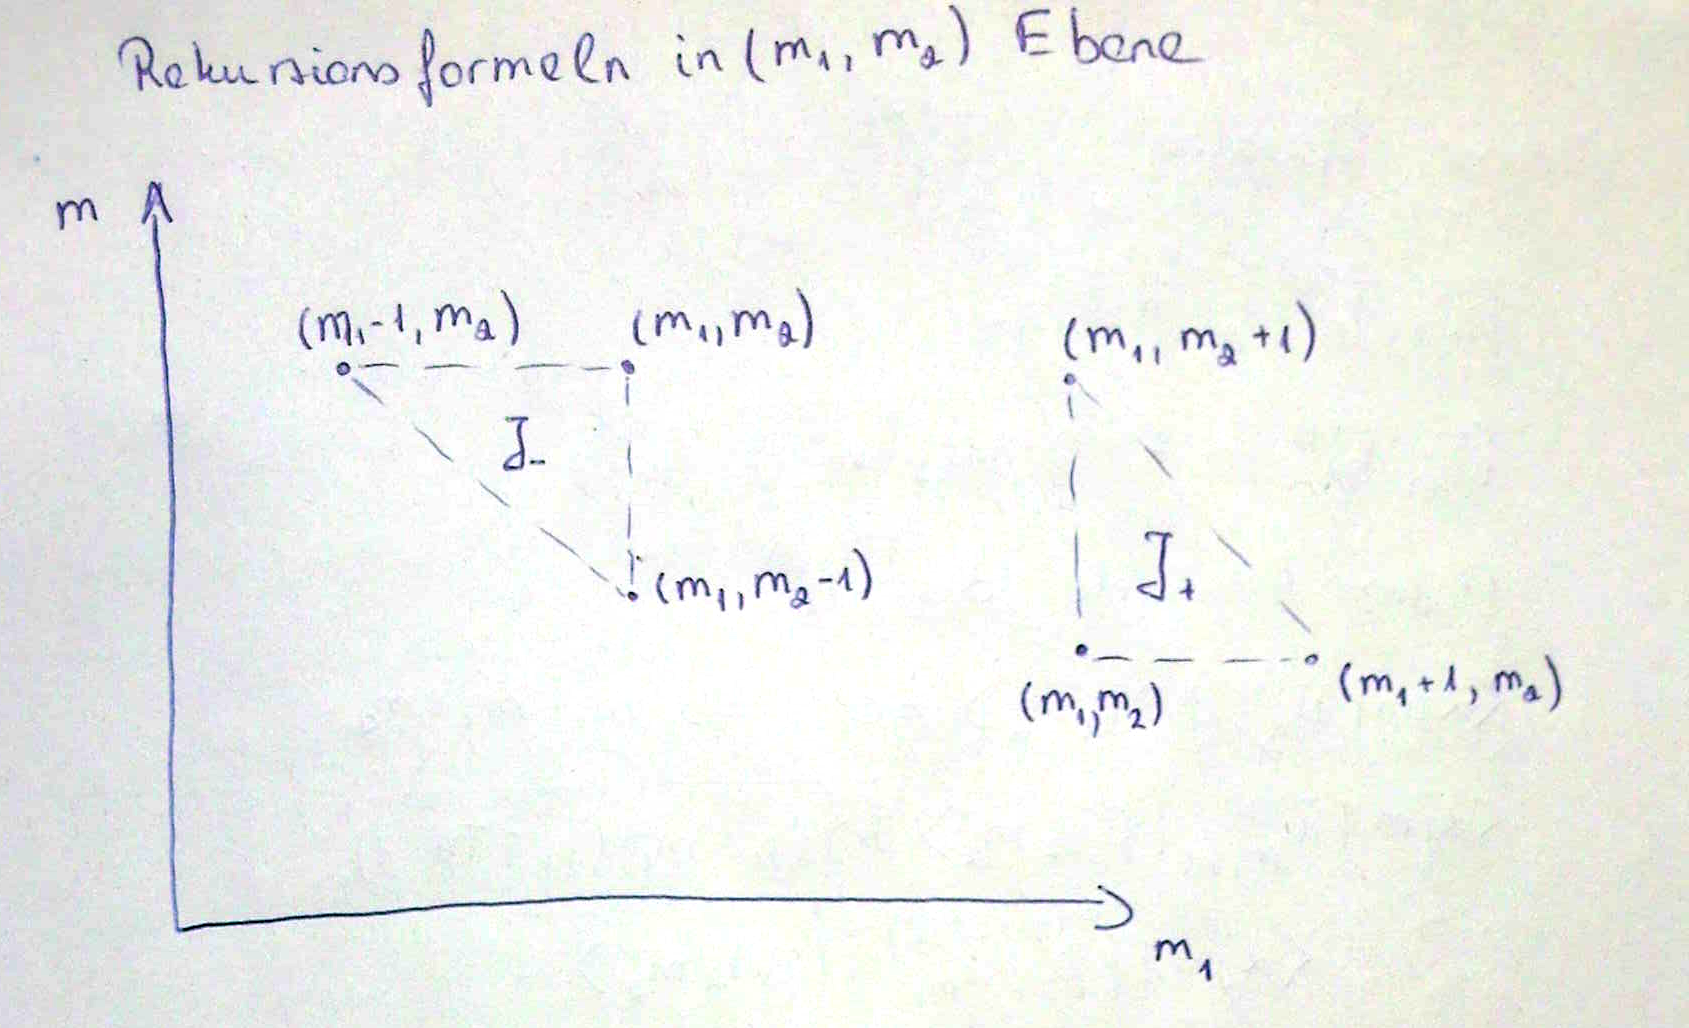
\includegraphics[width=0.75\textwidth]{09_01.png}

pic 2
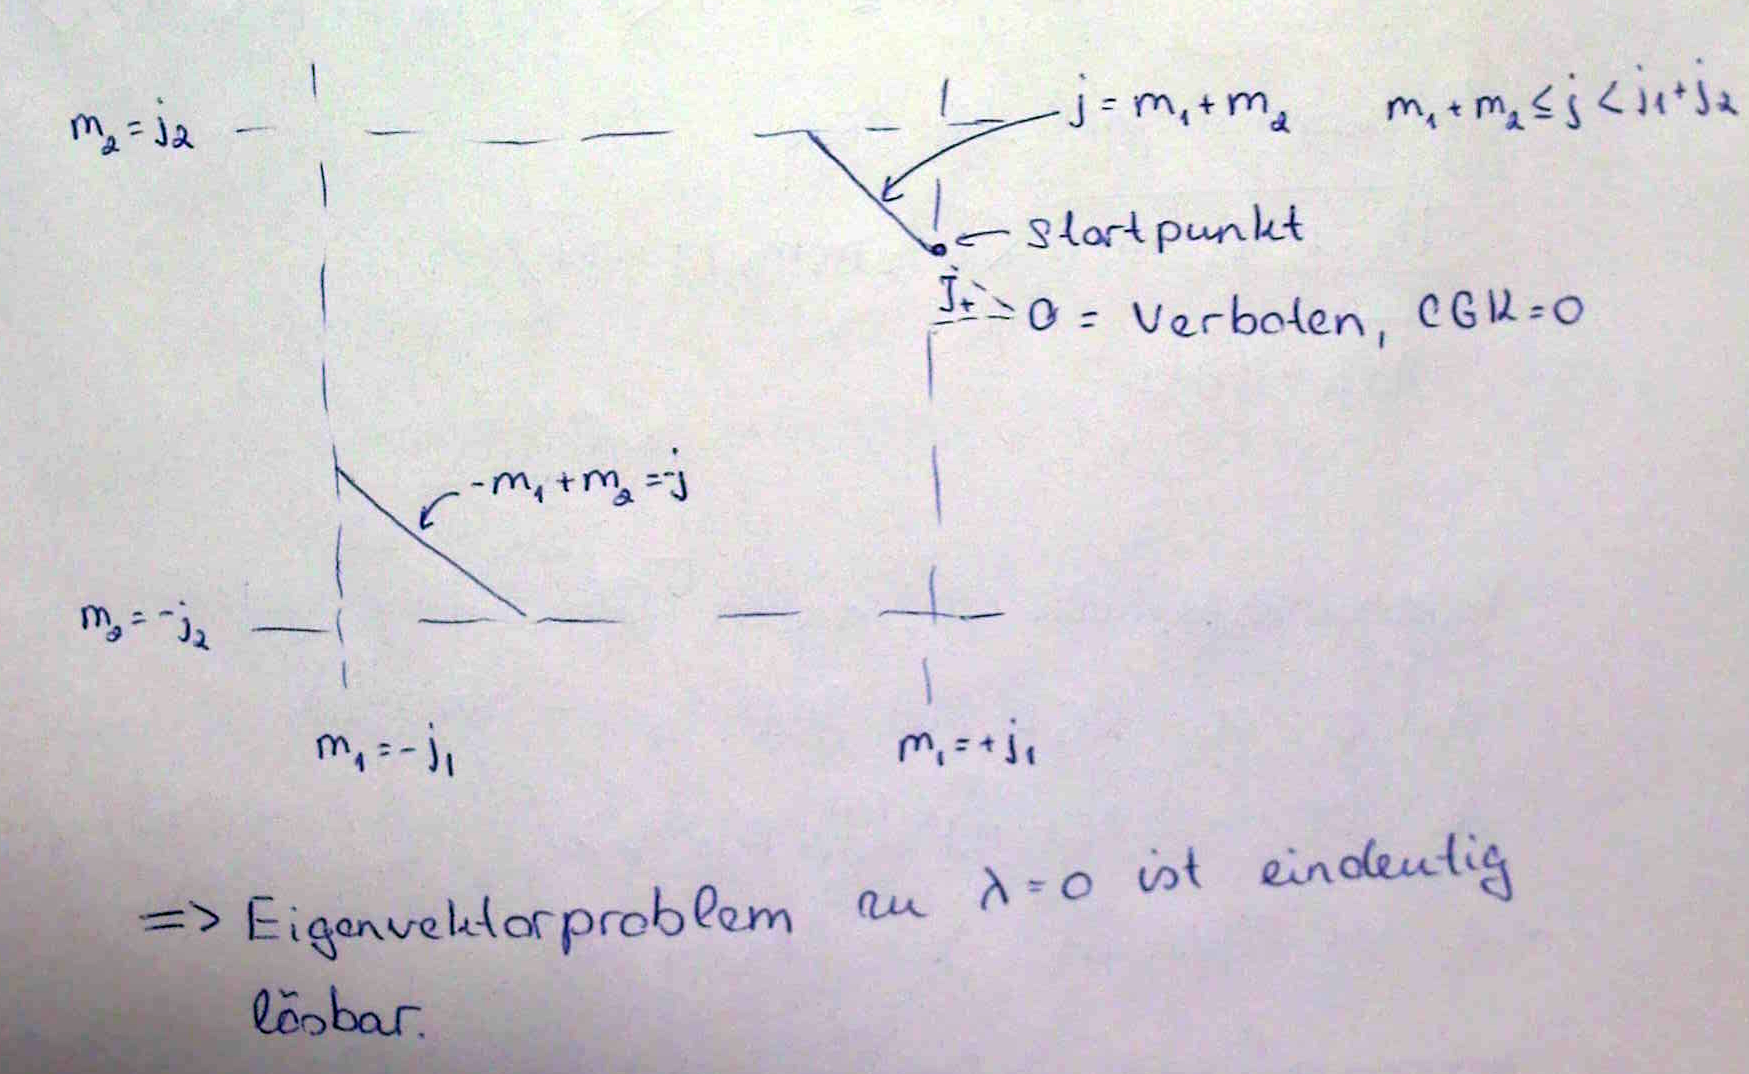
\includegraphics[width=0.75\textwidth]{09_02.png}

\(\Rightarrow\) Eigenvektorproblem zu \(\lambda = 0\) ist eindeutig lösbar
\(x=c_1z\), \(y=c_2=z\) : \(y=c_2 \frac x {c_1} = \frac {c_2}{c} x\)

\[ y_i = \langle \alpha jm|T^{(j_1)}_{m_1}|\beta j_2 m_2\rangle =
\frac {c_2}{c_2}  \langle j_1j_2, m_1m_2| jm\rangle\]

Schreibweise für \(\frac {c_2}{c_2}\)

\[\frac {c_2}{c_2} = \frac {\langle \alpha j||T^{(j_1)}||\beta  j_2\rangle}{\sqrt{2j_2+1}}\]

\(\frac {c_2}{c_2}\) ist unabhängig von \(m_1,m_2,m\) !

\subsection{Wigner-Eckart Theorem}

\(\langle \alpha j||T^{(j_1)}|| \beta j_2\rangle \) heißt reduziertes
  Matrixelement.

a) Auswahlregel:   \(\langle \alpha jm|T^{(j_1)}_{m_1}|\beta j_2 m_2\rangle\neq 0\) \(\Rightarrow m= m_1+m_2\);  \(j_1+j_2 \geq j\geq |j_1-j_2|\)

Beispiel: Ortsoperator \(\vec r\) (Dipolübergänge) trägt \(j_1=1\)

\(\Rightarrow \langle \alpha jm|\vec r|\beta j_2 m_2\rangle \neq 0\)
\(\Rightarrow j=j_2, j_2\pm 1 (j_2\neq 0)\)

b) Auswahlregel \(\langle \alpha' j=0, m=0|T^{(1)}_{m}|\beta j=0
m=0\rangle = 0\) kein \(j=0 \rightarrow j=0\) Übergang durch Dipolübergang

\subsection{Projektionstheorem für Vektoroperatoren}
Sie \(V_q(q=\pm 1, 0)\) ein Vektrooperator, Dann gilt:

\[\langle \alpha' jm'|V_q|\alpha j m\rangle 
= \frac{\langle \alpha jm|\vec J\cdot \vec V|\alpha j m\rangle}{\hbar^2 j(j+1)} \langle jm'|J_q| j m\rangle \]

mit \(J_{\pm 1}= \mp \frac {1}{\sqrt 2} (J_x\pm J_y) = \mp  \frac {1}{\sqrt 2} J_\pm\) , \(J_0=J_z\)

Beweis: Betrachtej\(\langle \alpha jm|\underbrace{\vec J\cdot \vec V}_{J_0V_0-J_{+1}V_{-1}-J_{-1}V_{+1}}|\alpha j m\rangle \)
mit \(J_0V_0-\underbrace{J_{+1}}_{-\frac {1}{\sqrt 2}J_+}V_{-1}-\underbrace{J_{-1}}_{\frac {1}{\sqrt 2}J_-}V_{+1}\)

\[=\left( \langle \alpha' jm| \hbar m V_0 + \frac {1}{\sqrt 2}\hbar
  \sqrt{(j+ m)(j-m+1)} \rangle \alpha' j m-1|V_{-1} -  \frac {1}{\sqrt 2}\hbar
  \sqrt{(j- m)(jm+1)} \rangle \alpha' j m+1| V_{+1} \right) |\alpha jm \]


\[ = c (j,m)  \langle \alpha'j||V||\alpha j\rangle \]

\(\vec J\cdot \vec V\) ist Skalar, d.h. hat \(j_1=0\)

\[\Rightarrow \langle \alpha jm|\vec J\cdot \vec V|\alpha jm\rangle =
\underbrace{\langle j 0; m 0 |jm\langle}_{1} \frac{\langle \alpha' j||\vec J\cdot \vec V|\alpha j\rangle}{\hbar^2 j(j+1)} 
\]

\(\Rightarrow c(\underbrace{j}_{c_j},m)\) hängt nicht von m ab! und
nicht von \(V_q,\alpha,\alpha\)

Wähle \(V_q=J_q\) um \(c_j\) zu berechnen

\[ c_j\langle \alpha j||J||\alpha j\rangle = \langle \alpha jm|\underbrace{\vec J^2}_{\hbar^2 j(j+1)}|\alpha jm\rangle = \hbar^2j(j+1)\]


Wigner Eckart Theorem

\[\langle \alpha' jm'|V_q|\alpha jm\rangle = 
\underbrace{\frac{ \langle jm'| \overbrace{jj}^{?}; mq\rangle}{\sqrt{2j+1}}}_{(*)} \langle \alpha' j|| V || \alpha j\rangle
\]

\[ (*) \frac{ \langle jm'| \overbrace{jj}^{?}; mq\rangle}{\sqrt{2j+1}}
= \frac{ \langle \alpha jm'| J_q|\alpha jm\rangle}{\langle \alpha j||J|| \alpha j \rangle} \cdot 
\frac{ \langle \alpha' jm| \vec J \cdot \vec V|\alpha jm\rangle}{c_j}
\]

\[ =\langle \alpha' jm| \vec J \cdot \vec V|\alpha jm\rangle \langle jm'|J_q| \alpha jm\rangle \frac 1 {\hbar^2 j(j+1)} \qquad q.e.d\]

Matrixelemente von \(J_q\)

\[ \langle \alpha jm'| \underbrace{J_0}_{=J_z} |\alpha jm\rangle =\hbar m \delta_{mm'}\]

\[ \langle \alpha jm'| \underbrace{J_{\pm 1}}_{\mp\frac 1 {\sqrt2}J_\pm} |\alpha jm\rangle = \mp\frac 1 {\sqrt 2} \hbar
\sqrt{(j\mp m)(j\pm m+1)}\delta_{m',m\pm 1} 
\]





\end{document}
